\section{GSM - Gleichstrommotoren}

\vspace{-0.5cm}
\begin{minipage}[b]{0.45\textwidth}
	\centering
	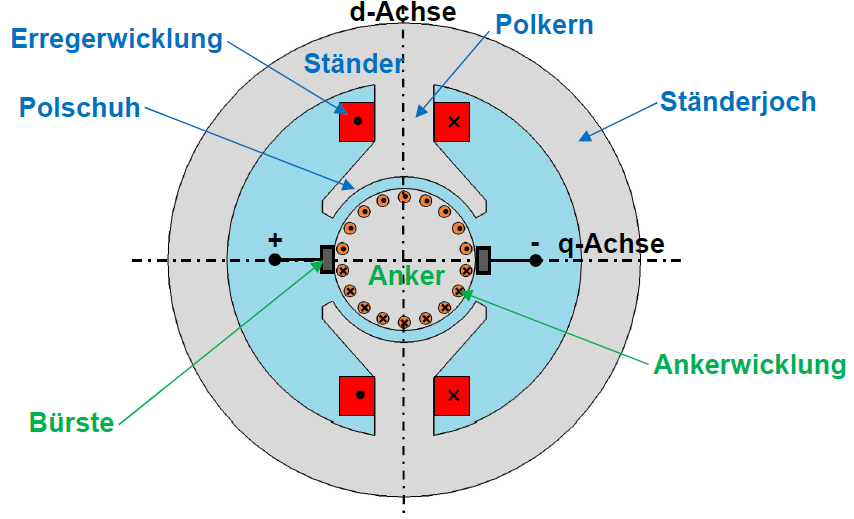
\includegraphics[width=8cm]{images/GSM_Aufbau.png}
\end{minipage}
\begin{minipage}[b]{0.25\textwidth}
	\centering
	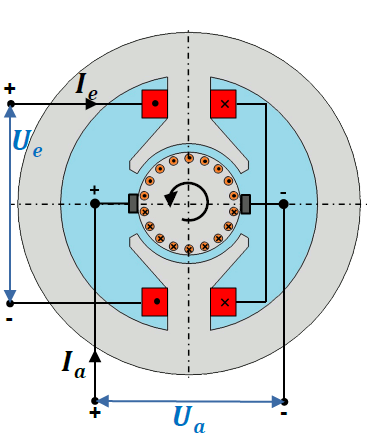
\includegraphics[width=5cm]{images/Grundgleichungen.png}
	\vspace{-1cm}
\end{minipage}
\begin{minipage}[b]{0.33\textwidth}
	\vspace{-2cm}
	\centering
	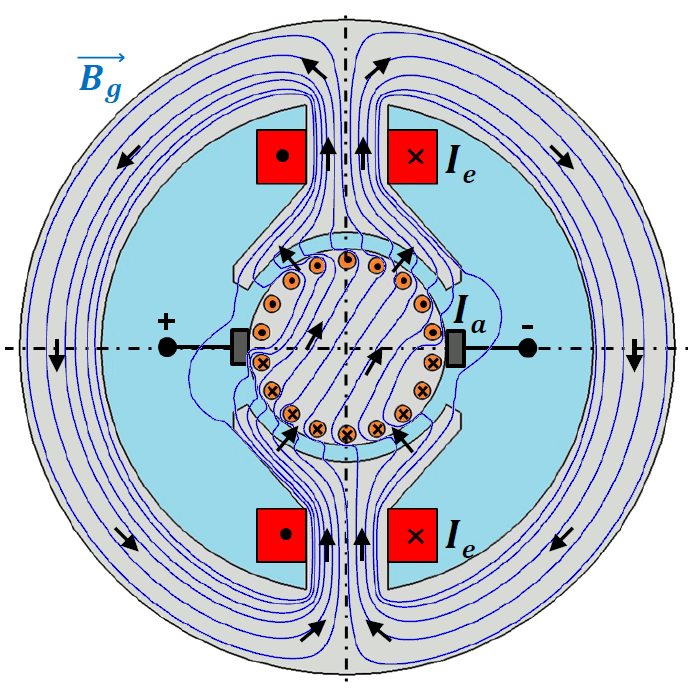
\includegraphics[width=5cm]{images/Ankerrueckwirkung.png}
	\vspace{0.2cm}
\end{minipage}
\vspace{-1cm}

\subsection{Fremderregte GSM}
\vspace{-0.2cm}
\begin{minipage}[b]{0.5\textwidth}
	\raggedright
	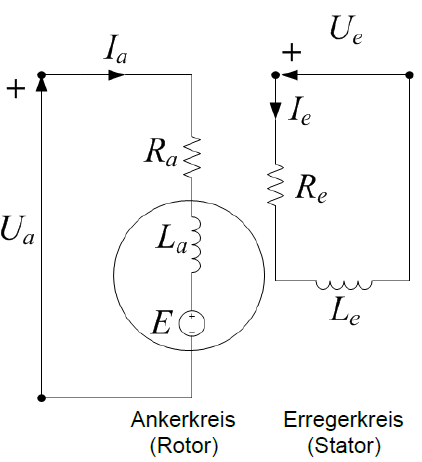
\includegraphics[width=6cm]{images/Ersatzschaltbild_GSM.png}
\end{minipage}
\begin{minipage}[b]{0.5\textwidth}
	\raggedright
	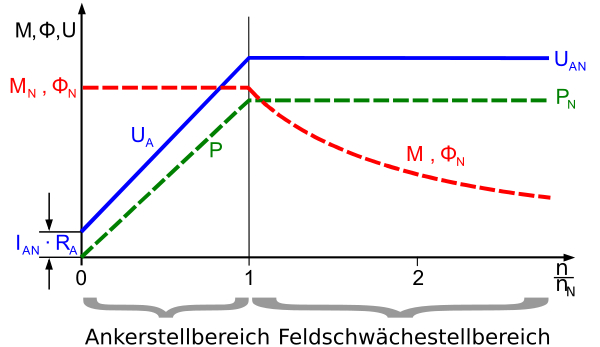
\includegraphics[scale = 0.7]{images/KennlinieFremderregt}
\end{minipage}\\

\begin{longtable}{| p{.25\textwidth} | p{.40\textwidth} | p{.30\textwidth} |}
    \firsthline
    \textbf{Erregerwicklung}	&
    $U_e = R_e\cdot I_e + L_e\cdot\dfrac{dI_e}{dt}$ &
    Spannungsgleichung des Statorkreises
    \\ \hline
    
    \textbf{Ankerwicklung}	&
    \[ U_a = R_a \cdot I_a + L_a \cdot \dfrac{dI_a}{dt} + E \] &
    $E = \omega\cdot\psi$
    \qquad $\psi = L_e\cdot I_e \, \widehat{=}$ Erregerfluss \newline \newline
    $\omega = 2\pi\cdot n$ \newline
    \quad n $\widehat{=}$ Drehzahl des Läufers $\left[\dfrac{1}{s}\right]$\newline \newline Spannungsgleichung des Rotorkreises
    \\ \hline
    
    \textbf{Elektrische Leistung} &
    Im stationären Betrieb: \quad $\left(\dfrac{d}{dt} = 0\right)$ \newline \newline
    $P_{el} = P_e + P_a = U_e\cdot I_e + U_a\cdot I_a$ \newline \newline
    $P_{el} = \underbrace{R_e\cdot I_e^2}_{\substack{Ohmsche \\ Erregerverluste}} + \underbrace{R_a\cdot I_a^2}_{\substack{Ohmsche \\ Ankerverluste}} + \underbrace{\omega\cdot\psi\cdot I_a}_{\substack{Mechanische\\Leistung}}$ \newline &
    $[P] = W$
    \\ \hline
    
    \textbf{Mechanische Leistung} &
    $P_{mech} = \omega\cdot M = \omega\cdot\psi\cdot I_a\, = \omega\cdot L_e \cdot I_e \cdot I_a$ &
    \\ \hline
    
    \textbf{Drehmoment} &
    $M = \psi\cdot I_a\, = L_e\cdot I_e\cdot I_a$ &
    $[M] = Nm$
    \\ \lasthline
\end{longtable}
\clearpage
\newpage

\subsection{Nebenschluss GSM}
Die Erreger- und Ankerwicklung werden parallel an die gleiche Spannungsquelle geschaltet.\newline Beim Nebenschluss sind die Anker- und Erregerspannung gleich und der Anker- und Erregerstrom unabhängig \newline voneinander. \\
\begin{minipage}[b]{0.4\textwidth}
	\raggedright
	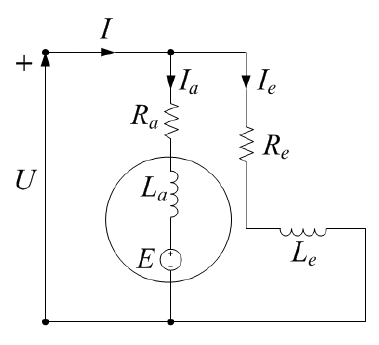
\includegraphics[width=6cm]{images/Nebenschluss_GSM.png}
\end{minipage}
\begin{minipage}[b]{0.5\textwidth}
	\raggedright
	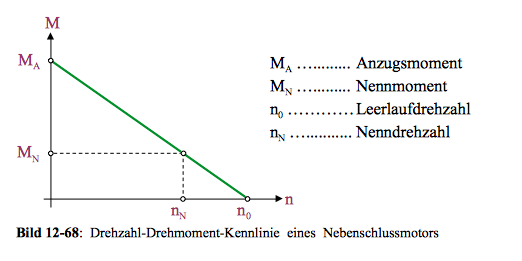
\includegraphics[scale = 0.6]{images/KennlinieNebenschluss}
\end{minipage}\\

%\renewcommand{\arraystretch}{2.5}
\begin{longtable}{| p{.25\textwidth} | p{.40\textwidth} | p{.30\textwidth} |}
	\firsthline
	\textbf{Drehmoment}	&
    $U = U_a = R_a\cdot I_a + \omega\cdot\psi$ \newline \newline
    $I_a = \dfrac{U - \omega\cdot\psi}{R_a}$ \newline \newline
    $M = I_a\cdot\psi\, = \, I_a \cdot L_e \cdot I_e $ \newline\newline
    $M = \dfrac{U\cdot\psi}{R_a}-\dfrac{\omega\cdot\psi^2}{R_a}$ \newline &
    Spannungsgleichung der Nebenschluss-Schaltung\newline \newline
    $\psi = L_e\cdot I_e \, \widehat{=}$ Erregerfluss \newline \newline
    $\omega\, = \, 2\pi\cdot n \quad \left[\dfrac{1}{s}\right]$
    \\ 	\hline
    
	\textbf{Anlaufmoment} \newline \newline
    $(n = 0)$	&
    $M_A = \dfrac{U\cdot\psi}{R_a + R_v}$ \newline \newline
    $I_{Anlauf} \,= \, \dfrac{U}{R_a + R_v} $ &
    $[M] = Nm$ \newline
    $R_a \, \widehat{=}$\, Ankerwiderstand \newline
    $R_v \, \widehat{=}$ Im Ankerkreis in Serie geschalteter Regelungswiderstand (= \textbf{oft 0})
    \\ \hline
    
	\textbf{Elektrische Leistung} &
    Im stationären Betrieb: \quad $\left(\dfrac{d}{dt} = 0\right)$ \newline \newline
    $P_{el} = P_e + P_a = U_e\cdot I_e + U_a\cdot I_a$ \newline \newline
    $P_{el} = \underbrace{R_e\cdot I_e^2}_{\substack{Ohmsche \\ Erregerverluste}} + \underbrace{R_a\cdot I_a^2}_{\substack{Ohmsche \\ Ankerverluste}} + \underbrace{\omega\cdot\psi\cdot I_a}_{\substack{Mechanische\\Leistung}}$ \newline &
    $[P] = W$
    \\ \hline
    
	\textbf{Mechanische Leistung} &
    $P_{mech} = \omega\cdot M = \omega\cdot\psi\cdot I_a$ &
    \\ \hline
    
	\textbf{Leerlaufdrehzahl}&
    $n_0 = \dfrac{U}{2\pi\cdot\psi}$  \qquad $(M = 0)$&
    $[n] = \dfrac{1}{s}$
    \\ \lasthline
\end{longtable}
\clearpage
\newpage

\subsection{Reihenschluss GSM}
Die Erreger- und Ankerwicklung werden in Serie an die gemeinsame Spannungsquelle geschaltet.\newline Beim Reihenschluss sind die Anker- und Erregerströme gleich und die Anker- und Erregerspannungen sind deshalb \newline stark voneinander abhängig.\newline
\begin{minipage}[b]{0.4\textwidth}
	\raggedright
	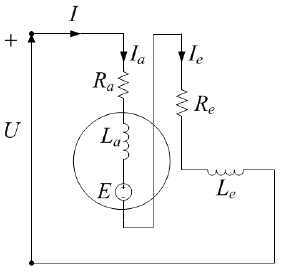
\includegraphics[width=6cm]{images/Reihenschluss.png}
\end{minipage}
\begin{minipage}[b]{0.5\textwidth}
	\raggedright
	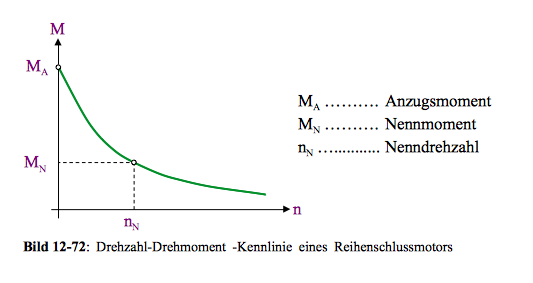
\includegraphics[scale = 0.6]{images/KennlinieReihenschluss}
\end{minipage}\\
\begin{minipage}[b]{0.7\linewidth}
    \raggedleft
    \textcolor{red}{Achtung: M $\rightarrow$ 0 $\Rightarrow$ n $\rightarrow \infty$}
\end{minipage}
\\

\begin{longtable}{| p{.25\textwidth} | p{.40\textwidth} | p{.30\textwidth} |}
	\firsthline
	\textbf{Drehmoment}	&
    $U = (R_a + R_e)\cdot I + 2\pi n\cdot\psi$ \newline \newline
    $M = I\cdot\psi$ \newline \newline
    $M = I\cdot\psi = L_e\cdot\left(\dfrac{U}{R_a + R_e + 2\pi n\cdot\psi}\right)^2$\newline\newline
    $\psi = L_e\cdot I$ & Spannungsgleichung der Reihenschluss-Schaltung \newline \newline $I\,=\,I_a\,=\,I_e$
    \\\hline
    
	\textbf{Anlaufmoment}	&
    $M_A = \dfrac{L_e\cdot U^2}{\left(R_a + R_e\right)^2}$ \qquad $\left(n = 0\right)$ &
    $[M] = Nm$ 
    \\ \hline
    
	\textbf{Bezugsdrehzahl}&
    $n_b = \dfrac{R_a + R_e}{2\pi\cdot L_e}$ \newline &
    $[n] = \dfrac{1}{s}$
    \\ \lasthline
\end{longtable}

\subsection{Drehzahlregelung}
\begin{minipage}[b]{0.33\textwidth}
	\raggedright
	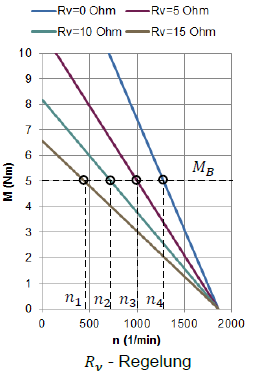
\includegraphics[width=5cm]{images/Widerstandsregelung.png}
\end{minipage}
\begin{minipage}[b]{0.33\textwidth}
	\raggedright
	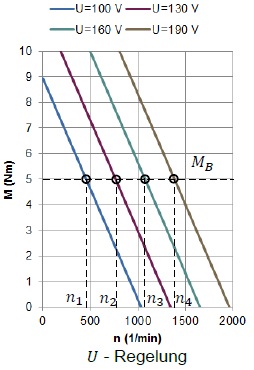
\includegraphics[width=5cm]{images/Spannungsregelung.png}
\end{minipage}
\begin{minipage}[b]{0.33\textwidth}
	\raggedright
	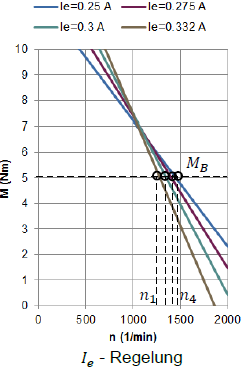
\includegraphics[width=5cm]{images/Erregerstromregelung.png}
\end{minipage}
\clearpage
\newpage






